

\documentclass[aspectratio=169]{beamer}
\usepackage[utf8]{inputenc}
%\usepackage[latin1]{inputenc}
%\usepackage[cyr]{aeguill}
\usepackage[T1]{fontenc}
\usepackage{graphicx}
\usepackage{amsmath,amsfonts,amsthm,amssymb}
\usepackage{algorithm}
\usepackage{algorithmic}
\usepackage{fancyhdr}
%\usepackage[]{algorithm2e}
%\usepackage{hyperref}
\usepackage{color}
\usepackage{pstricks}
%\usepackage{stmaryrd}
%\usepackage{enumitem} 
\usepackage{bbm}
\usepackage{bm}
%\usepackage{showlabels}
\usepackage{cases}
\usepackage{array}
\usepackage{relsize,exscale}
\usepackage{caption}
\usepackage{times}
\usepackage{subcaption}
\usepackage{graphicx} 
\usepackage{epstopdf}
\usepackage{tikz}
\usepackage{glossaries}


\setbeamersize{text margin left=0.2 cm}
  \setbeamersize{text margin right=0.2 cm}
  %\setbeamersize{sidebar width left=}
  %\setbeamersize{sidebar width right=taille}
%\usetikzlibrary{calc}
%\DeclareMathOperator*{\argmin}{argmin}

\definecolor{ao(english)}{rgb}{0.0, 0.5, 0.0}
\definecolor{armygreen}{rgb}{0.29, 0.33, 0.13}
\definecolor{britishracinggreen}{rgb}{0.0, 0.26, 0.15}
\definecolor{cadmiumgreen}{rgb}{0.0, 0.42, 0.24}
\definecolor{indigo}{rgb}{0.29, 0.0, 0.51}
\definecolor{lightgray}{gray}{0.85}
\definecolor{midnightblue}{rgb}{0.1, 0.1, 0.44}
\definecolor{burntorange}{rgb}{0.8, 0.33, 0.0}
\definecolor{royalblue}{rgb}{0.25, 0.41, 0.88}
\definecolor{darkmagenta}{rgb}{0.55, 0.0, 0.55}
\definecolor{byzantine}{rgb}{0.74, 0.2, 0.64}
\definecolor{blue-violet}{rgb}{0.54, 0.17, 0.89}
\definecolor{brown-traditional}{rgb}{0.59, 0.29, 0.0}
\definecolor{brown-web}{rgb}{0.65, 0.16, 0.16}
\definecolor{burgundy}{rgb}{0.5, 0.0, 0.13}
\definecolor{electricpurple}{rgb}{0.75, 0.0, 1.0}
\definecolor{gray}{rgb}{0.5, 0.5, 0.5}
\definecolor{goldenbrown}{rgb}{0.6, 0.4, 0.08}
\definecolor{armygreen}{rgb}{0.29, 0.33, 0.13}
\definecolor{calpolypomonagreen}{rgb}{0.12, 0.3, 0.17}
\definecolor{caputmortuum}{rgb}{0.35, 0.15, 0.13}
\definecolor{carmine}{rgb}{0.59, 0.0, 0.09}
\definecolor{chocolate-traditional}{rgb}{0.48, 0.25, 0.0}
\definecolor{lincolngreen}{rgb}{0.11, 0.35, 0.02}
\definecolor{magenta}{rgb}{1.0, 0.0, 1.0}
\definecolor{auburn}{rgb}{0.43, 0.21, 0.1}
\definecolor{bole}{rgb}{0.47, 0.27, 0.23}
\definecolor{bulgarianrose}{rgb}{0.28, 0.02, 0.03}
%\graphicspath{{./Figures/}}
\newtheorem{assumption}[theorem]{Assumption} 
\newtheorem{proposition}[theorem]{Proposition} 
\newtheorem{remark}[theorem]{Remark} 

\renewcommand{\div}{\mathrm{div}}
\newcommand{\Pdot}{\ddot{P}}
\newcommand{\Pdothn}{\Pdot_h^n}
%\usetheme{Madrid}
\usetheme{Frankfurt}
\vspace*{-0.7 cm}
\title{High-order numerical
discretizations and a posteriori error estimates for variational inequalities}
\author{\underline{\textbf{JAD DABAGHI}}}

\institute[]{Sorbonne Université (LJLL) \& CEA Paris Saclay }
\date{Seminar of Modeling, Analysis $\&$ Simulation, MAP5, February $5^{\mathrm{th}}$ 2021}
\input{manuscrit_commandes}

\setbeamertemplate{navigation symbols}{}
\setbeamercovered{transparent}


\AtBeginSection[] {
    \begin{frame}
    <beamer>[noframenumbering]
        \frametitle{Outline}
        \tableofcontents[currentsection]
    \end{frame}
}


\newcommand{\kk}{\textcolor{royalblue}{k}}
\newcommand{\ii}{\textcolor{burntorange}{i}}
\newcommand{\nuu}{\textcolor{burntorange}{\nu}}
\newcommand{\zzero}{\textcolor{royalblue}{0}}
\newcommand{\izzero}{\textcolor{burntorange}{0}}
\begin{document}

\addtobeamertemplate{footline}{\hfill\insertframenumber/\inserttotalframenumber\hspace{1em}\null}



\begin{frame}
\maketitle
\includegraphics[scale=0.2]{logo_sorbonne}
\hfill 
\includegraphics[scale=0.13]{CEA}

\end{frame}


%% INTRODUCTION

\section{Introduction}
\subsection{}
%\setbeamertemplate{footline}[frame number]
\begin{frame}
\frametitle{Motivation}
$\Omega \subset \mathbb{R}^2$: smooth connected domain,
$\mathcal{H}$ : Hilbert space, $\mathcal{K}_g$ : convex set.
\\
\vspace*{0.1 cm}
$a: \mathcal{H} \times \mathcal{H} \rightarrow \mathbb{R}$: bilinear continuous  coercive form, $\ell : \mathcal{H} \rightarrow \mathbb{R}$ : linear continuous form
\begin{equation*}
\text{Find} \quad \textcolor{red}{u} \in \mathcal{K}_g \quad a(\textcolor{red}{u},v-\textcolor{red}{u}) \geq \ell(v-\textcolor{red}{u}) \quad \forall v \in \mathcal{K}_g
\end{equation*}
\invisible<1>{
\textcolor{cadmiumgreen}{\textbf{Application to several problems in contact mechanics}}
\\
\vspace*{0.2 cm}
\invisible<2>{
\textcolor{midnightblue}{\textbf{Obstacle problem:}}
Find $\textcolor{red}{u} \in \Kg := \left\{ v \in H^1(\Omega) \ \text{s.t.} \ v=g \ \text{on} \ \partial \Omega , \ \text{and} \ v \geq \Psi \ \text{in} \ \Omega \right\}$ such that
\begin{equation*}
\left( \nab \textcolor{red}{u}, \nab (v-\textcolor{red}{u}) \right)_{\Omega} \geq \left(f,v-\textcolor{red}{u}\right)_{\Omega} \quad \forall v \in \Kg
\end{equation*}
\vspace*{-0.2 cm}
\begin{minipage}{0.55\linewidth}
\begin{itemize}
\item $\textcolor{red}{u}$: displacement of an elastic membrane
  \item $\Psi \in H^1(\Omega)$: position of the lower obstacle 
  \item $g \in H^{\frac{1}{2}}(\partial \Omega)$: Dirichlet boundary datum for $\textcolor{red}{u}$
    \item $f \in L^2(\Omega)$: force acting on the membrane
\end{itemize}
\end{minipage}
\hfill
\begin{minipage}{0.4\linewidth}
\includegraphics[scale=0.3]{image_obstacle}
\end{minipage}

\invisible<3>{
}}}
\end{frame}
%%%%%%%%%%%%
\begin{frame}
  \textcolor{midnightblue}{\textbf{Signorini problem:}}
  $\partial \Omega = \Gamma_{\mathrm{D}} \cup \Gamma_{\mathrm{N}} \cup \Gamma_{\mathrm{C}}$. \\
  $\Gamma_{\mathrm{D}}$: Dirichlet boundary conditions, $\Gamma_{\mathrm{N}}$: Neumann boundary conditions \\
  $\Gamma_{\mathrm{C}}$: Unilateral contact boundary conditions
  \\
  \vspace*{0.1 cm}
  Find $\textcolor{red}{\bu} \in \Kg := \left\{ \bv \in [H^1(\Omega)]^2 \ \text{s.t.} \ \bv=g \ \text{on} \ \Gamma_{\mathrm{D}}, \ \text{and} \ \bv\cdot \bn \leq 0 \ \text{on} \ \Gamma_{\mathrm{C}} \right\}$ such that
\begin{equation*}
\left( \sigma (\textcolor{red}{\bu}), \epsilon (\bv-\textcolor{red}{\bu}) \right)_{\Omega} \geq \left(\bbf,\bv-\textcolor{red}{\bu}\right)_{\Omega} + \left({\bm g}_{N}, \bv-\textcolor{red}{\bu} \right)_{\Gamma_{\mathrm{N}}}\quad \forall \bv \in \Kg
\end{equation*}

\begin{minipage}{0.55 \linewidth}
\begin{itemize}
\item $g \in H^{\frac{1}{2}}(\Gamma_{\mathrm{D}})$ : Dirichlet boudary datum for $\textcolor{red}{u}$
  \item  ${\bm g}_{\mathrm{N}} \in [L^2(\Gamma_{\mathrm{N}})]^2$ :  Neumann boundary data
  \item  $f \in [L^2(\Omega)]^2$: force acting on the solid elastic.
\end{itemize}
\end{minipage}
\hfill
\begin{minipage}{0.42 \linewidth}
\includegraphics[scale=0.4]{image_signorini}
\end{minipage}
\end{frame}
\begin{frame}
\textcolor{midnightblue}{\textbf{Contact between two membranes:}}
\\
\vspace*{0.1 cm}
Find $\textcolor{red}{\bu}:=(\textcolor{red}{u_1},\textcolor{red}{u_2}) \in \Kg := \left\{ \bv = \left(v_1,v_2\right) \in H_{g_1}^1(\Omega) \times H_{g_2}^1(\Omega) \ \text{s.t.} \ v_1 - v_2 \geq 0  \ \text{a.e.} \ \text{in} \ \Omega \right\}$ such that
 \begin{equation*}
  \fbox{$ \sum_{\alpha=1}^2 \mu_{\alpha}
   \left( \nab \textcolor{red}{u_{\alpha}}, \nab \left(v_{\alpha} - \textcolor{red}{u_{\alpha}} \right) \right)_{\Omega} \geq
   \sum_{\alpha=1}^2 \left(f_{\alpha}, v_{\alpha} - \textcolor{red}{u_{\alpha}} \right)_{\Omega} \quad \forall \bv \in \Kg$ }
 \end{equation*}
 \begin{minipage}{0.37 \linewidth}
 \begin{itemize}
 \item $\mu_1, \mu_2$: tensions of the membranes
   \item $g_1 \geq g_2$ : boundary data
\end{itemize} 
 \end{minipage}
 \hfill
 \begin{minipage}{0.55 \linewidth}
\begin{figure}
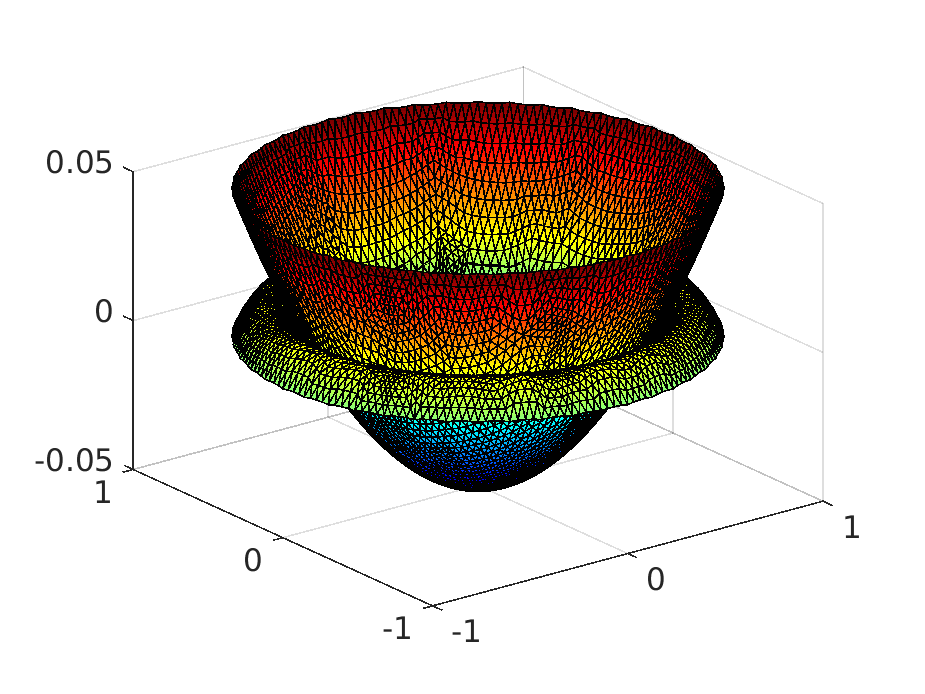
\includegraphics[scale = 0.5]{fig_article_chap_1/fig_membrane_cv.eps}    
\end{figure}
\end{minipage}

 \end{frame}
%%%%

%%%%%%%%%%%%%%%%%
\begin{frame}
\vspace*{0.1 cm}
\textcolor{red}{\textbf{Study the contact problem between two membranes}}
\\
\vspace{0.3 cm}
\textcolor{cadmiumgreen}{\textbf{Propose robust algorithms}}
\begin{itemize}
\item Discretization by the finite element method, the discontinuous Galerkin method, the hybrid high-order method
\end{itemize}
\textcolor{cadmiumgreen}{\textbf{Nonlinear resolution}}
\begin{itemize}
\item Semismooth Newton methods
  \end{itemize}
\textcolor{cadmiumgreen}{\textbf{Quantify the error}}
\begin{itemize}
  \item A posteriori error estimates
  \item Distinction of each error components
\end{itemize}

\textcolor{cadmiumgreen}{\textbf{Save computational time}}
\begin{itemize}
\item Adaptivity
  \end{itemize}
  \invisible<1>{
  \textcolor{red}{\textbf{Extension to unsteady problems?}}
  \invisible<2>{
  }}
\end{frame}




%%%%%%%%%%%%%%%%%%%%%%%%%%%%%
%% CHAP 1

\section{Model problem and discretization}
\subsection{}

\input{Part1}

%%%% CHAP 2

\section{A posteriori analysis}
\subsection{}


\begin{frame}
  %%%%%%%%%%%%%%%%%%%
\frametitle{A posteriori analysis for finite elements}
\textcolor{cadmiumgreen}{\textbf{Goal:}}
\begin{equation*}
\tnorm{\bu-\bu_h^{\kk,\ii}}_{\Omega} \egaldef \left(\sum_{\ialf = 1}^2 \mu_\ialf \left\|\nab \left(\uialf-\uialfh^{\kk,\ii} \right)\right\|_{\Omega}^2 \right)^{\frac{1}{2}} \leq \eta^{\kk,\ii} \egaldef \left(\sum_{K \in Th}\left[\eta_{K}(\bu_h^{\kk,\ii}) \right]^2\right)^{\frac{1}{2}}
\end{equation*}
\begin{itemize}
\item $\eta_{K}(\bu_h^{\kk,\ii})$ local estimator depending on the approximate solution 
\item $\eta^{\kk,\ii} \leq \eta_{\mathrm{disc}}^{\kk,\ii} + \eta_{\mathrm{lin}}^{\kk,\ii} + \eta_{\mathrm{alg}}^{\kk,\ii}$: identification of the error components
\item $\eta_{K}(\bu_h^{\kk,\ii}) \leq$ local error + $\underbrace{\mathrm{local \ contact \ term}}_{\mathrm{\textcolor{midnightblue}{typically \ very \ small}}}$: local efficiency
\item adaptive inexact stopping criteria based on the error components
\end{itemize} 
\invisible<1>{
\textcolor{red}{We employ the methodology of equilibrated flux reconstruction to obtain local error estimators.}
\newline 
\footnotesize{Destuynder \& M\'etivet (1999) Braess \& Sch\"oberl (2008), Ern \& Vohral{\'{\i}}k (2013)}
\invisible<2>{
}}
\end{frame}
%

%%%
\begin{frame}
\frametitle{Component flux reconstruction}
\textcolor{cadmiumgreen}{\textbf{Motivation:}}
\begin{equation*}
-\mu_\ialf \nab u_{\ialf} \in \HdivOmeg,  \quad  -\mu_\ialf \nab u_{\ialf h}^{\kk,\ii} \not \in \HdivOmeg, \quad \nab {\cdot} \left(-\mu_\ialf \nab u_{\ialf h}^{\kk,\ii} \right) \neq f_\ialf -(-1)^{\ialf} \lambh^{\kk,\ii}
\end{equation*}
\invisible<1>{
\textcolor{cadmiumgreen}{\textbf{Flux reconstruction:}}
\begin{equation*}
{\bm \sigma}_{\ialf h}^{\kk,\ii} \in \HdivOmeg \quad \left(\nab {\cdot} {\bm \sigma}_{\ialf h}^{\kk,\ii}, 1 \right)_K = \left( f_\ialf -(-1)^{\ialf} \lambh^{\kk,\ii}, 1  \right)_K 
\end{equation*}
\invisible<2>{
\textcolor{cadmiumgreen}{\textbf{Decomposition of the flux:}}
\begin{equation*}
{\bm \sigma}_{\ialf h}^{\kk,\ii}  = {\bm \sigma}_{\ialf h, \mathrm{alg}}^{\kk,\ii} + {\bm \sigma}_{\ialf h, \mathrm{disc}}^{\kk,\ii}
\end{equation*}
\invisible<3>{
\textcolor{cadmiumgreen}{\textbf{Algebraic error flux reconstruction:}}
\begin{equation*}
{\bm \sigma}_{\ialf h, \mathrm{alg}}^{\kk,\ii} \in \HdivOmeg \quad \nab {\cdot} {\bm \sigma}_{\ialf h, \mathrm{alg}}^{\kk,\ii}=r_{\ialf h}^{\kk,\ii} \quad \mbox{where} \quad r_{\ialf h}^{\kk,\ii} \quad \mbox{is the functional representation of} \quad {\bm R}_{\ialf h}^{\kk,\ii}
\end{equation*}
\scriptsize{Pape{\v z}, R{\"u}de, Vohral{\'{\i}}k and Wohlmuth (2020).}
\newline
\invisible<4>{
\normalsize{\textcolor{cadmiumgreen}{\textbf{Discretization flux reconstruction:}}
\begin{equation*}
{\bm \sigma}_{\ialf h, \mathrm{disc}}^{\kk,\ii} \in \HdivOmeg \quad \left(\nab {\cdot} {\bm \sigma}_{\ialf h,\mathrm{disc}}^{\kk,\ii}, 1 \right)_K = \left( f_\ialf -(-1)^{\ialf} \lambh^{\kk,\ii} - r_{\ialf h}^{\kk,\ii}, 1  \right)_K
\end{equation*}
}
\invisible<5>{
}}}}}
\end{frame}
%
\begin{frame}
\frametitle{Discretization flux reconstruction}
  ${\bm \sigma}_{\ialf h, \mathrm{disc}}^{\kk,\ii,\ba}$ are the solution of mixed system on patches
\begin{equation*}
\begin{array}{lclcc}
\left({\bm \sigma}_{\ialf h, \mathrm{disc}}^{\kk,\ii,\ba}, \tauh\right)_{\omah}- \left(\gamma_{\ialf h}^{\kk,\ii,\ba},\nab {\cdot} \tauh\right)_{\omah}
&=& -\left(\mu_\ialf \psiha \nab u_{\ialf h}^{\kk,\ii,\ba}, \tauh \right)_{\omega_h^{\ba}}
&  \forall \tauh\in \Vspaceha, \\
\left(\nab {\cdot} {\bm \sigma}_{\ialf h, \mathrm{disc}}^{\kk,\ii, \ba}, q_{h}\right)_{\omah}
&=&\left(\tilde{g}_{\ialf h}^{\kk,\ii,\ba}, q_{h}\right)_{\omah}
&  \forall q_{h}\in \Qspaceha,
\end{array}
\end{equation*}
\begin{equation*}
\tildgialfhkia  : \mbox{\textcolor{cadmiumgreen}{depends on the approximate solution}} 
%\left(f_\ialf -(-1)^{\ialf} \tildlambhkia -\rialfhki \right) \psiha- \mu_\ialf \nab \uialfhki {\cdot} \nab \psiha
\end{equation*}
\begin{minipage}[c]{0.4 \linewidth}
For each vertex $ \ba \in \Vh$
\vspace{-0.2 cm}
\begin{equation*}
\begin{split}
  \Vspaceha \subset \HdivOmeg, \quad
 \Qspaceha  \egaldef \Pp(\omah) \\
 {\bm \sigma}_{\ialf h, \mathrm{disc}}^{\kk,\ii} & \egaldef \sum_{\ba \in \mathcal{V}_h} {\bm \sigma}_{\ialf h, \mathrm{disc}}^{\kk,\ii,\ba}
\end{split}
\vspace{-0.2 cm}
\end{equation*}

\invisible<1>{
}
\end{minipage}
\hfill
\begin{minipage}[c]{0.5 \linewidth}
\begin{figure}
  %\begin{overprint}
    %\onslide<1>\includegraphics[width=0.84\textwidth]{patch_alg_3.pdf}
    \includegraphics[width=0.7\textwidth]{patch_alg_5.pdf}
   % \end{overprint}
\end{figure}
\end{minipage}
\end{frame}
%%%%ALG FLUX RECONSTRUCTION
% \begin{frame}
% \frametitle{Algebraic flux reconstruction}
% \vspace*{-0.5 cm}
% \begin{equation*}
% \begin{array}{lclcc}
% \left({\bm \sigma}_{\ialf j,\mathrm{alg}}^{\kk,\ii,\ba}, \tauj\right)_{\omajminusun}-\left(\gamma_{\ialf j}^{\kk,\ii,\ba},\nab {\cdot} \tauj\right)_{\omajminusun} &=& 0 & \forall \tauj\in \Vspacejjmuna, \\
% \left(\nab {\cdot} {\bm \sigma}_{\ialf j,\mathrm{alg}}^{\kk,\ii,\ba}, q_{j}\right)_{\omajminusun}&=&\dps\left(\tilde{g}_{\ialf j}^{\kk,\ii,\ba}, q_{j}\right)_{\omajminusun} & \forall q_{j} \in \Qspacejjmuna,
% \end{array}
% \end{equation*}
% \vspace{-0.8 cm}
% \begin{minipage}[c]{.55 \linewidth}
% \vspace{-0.8 cm}
% \begin{equation*}
% \begin{split}
% \Vspacejjmuna &\egaldef \left\{ \tauj \in \RTp(\omajminusun),
% \ \tauj {\cdot} \nnomajminusun =0 \mbox{ on } \partial \omajminusun \right\}, \\
% \Qspacejjmuna &\egaldef \Pp^{0}({\omajminusun}), \ \ba \in \mathcal{V}_{j-1}^{\mathrm{int}}
% \end{split}
% \end{equation*}
% \vspace{-0.2 cm}
% \invisible<1-2>{
% \begin{equation*}
% \begin{split}
% \Vspacejjmuna & \egaldef\left\{ \tauj \in \RTp(\omajminusun),
% \ \tauj {\cdot} \nnomajminusun=0 \  \mbox{on} \ \partial \omajminusun \backslash \partial \Omega\right\},
% \\
% \Qspacejjmuna & \egaldef \Pp({\omajminusun}), \ \ba \in \mathcal{V}_{j-1}^{\mathrm{ext}}
% \end{split}
% \end{equation*}
% }
% \end{minipage}
% \hfill
% \begin{minipage}[c]{.42 \linewidth}
% \hspace{3 cm}
% \begin{figure}
%   \begin{overprint}
%     \onslide<1>\includegraphics[width=0.9 \textwidth]{patch_alg_1.pdf}
%     \onslide<2>\includegraphics[width=0.9 \textwidth]{patch_alg_2.pdf}
%     \onslide<3>\includegraphics[width=0.9 \textwidth]{patch_alg_2_bis.pdf}
%     \onslide<4>\includegraphics[width=0.9 \textwidth]{patch_alg_3.pdf}
%     \onslide<5->\includegraphics[width=0.9 \textwidth]{patch_alg_4.pdf} 
%     \end{overprint}
% \end{figure}
% \end{minipage}
% \vspace{-0.2 cm}
% \invisible<1-4>{
% \begin{equation*}
% {\bm \sigma}_{\ialf j,\mathrm{alg}}^{\kk,\ii} \egaldef \sum_{j=1}^{J} \sum_{\ba \in \mathcal{V}_{j-1}} {\bm \sigma}_{\ialf j,\mathrm{alg}}^{\kk,\ii,\ba}
% \end{equation*}
% }
% \end{frame}
%
%
\begin{frame}
\frametitle{Estimators}

\textcolor{cadmiumgreen}{\textbf{Violations of physical properties of the numerical solution}}
\begin{equation*}
{\bm \sigma}_{\ialf h}^{\kk,\ii} \neq -\nab \uialfh^{\kk,\ii}, \qquad \nab {\cdot} {\bm \sigma}_{\ialf h}^{\kk,\ii} \neq f_\ialf -(-1)^{\ialf} \lambh^{\kk,\ii}
\end{equation*}
\invisible<1>{
\textcolor{midnightblue}{\textbf{Flux estimator:}}
\begin{equation*}
\eta_{\mathrm{F},K,\ialf}^{\kk,\ii} \egaldef \left\|\mu_\ialf^{\frac{1}{2}} \nab u_{\ialf h}^{\kk,\ii}
+\mu_\ialf^{-\frac{1}{2}} {\bm \sigma}_{\ialf h}^{\kk,\ii}\right\|_{K},
\end{equation*}
\textcolor{midnightblue}{\textbf{Residual estimator:}}
\begin{equation*}
\eta_{\mathrm{R},K,\ialf}^{\kk,\ii} \egaldef \frac{h_K}{\pi} \mu_\ialf^{-\frac{1}{2}}
\left\|f_\ialf - \nab {\cdot} {\bm \sigma}_{\ialf h}^{\kk,\ii} -(-1)^{\ialf} \lambh^{\kk,\ii} \right\|_{K},
\end{equation*}
\invisible<2>{
}}
\end{frame}
%
\begin{frame}
\textcolor{cadmiumgreen}{ \textbf{Violations of the complementarity constraints}}\\
%% \textcolor{red}{p = 1:} \ \textcolor{midnightblue}{\textbf{at convergence: $(k,i) \rightarrow + \infty$}} 
%% \vspace{-0.1 cm}
%% \begin{equation*} 
%% (\uunh \hspace{-0.05 cm} - \hspace{-0.05 cm} \udeuxh)(\ba) \hspace{-0.05 cm} \geq \hspace{-0.05 cm} 0 \hspace{-0.05 cm} \Rightarrow \hspace{-0.05 cm} \uh \hspace{-0.05 cm} \in \hspace{-0.05 cm} \Kg, \hspace{0.1 cm} \lambh(\ba) \hspace{-0.05 cm} \geq \hspace{-0.05 cm} 0 \hspace{-0.05 cm} \Rightarrow \hspace{-0.05 cm} \lambh \hspace{-0.05 cm} \in \hspace{-0.05 cm} \Lambda, \hspace{0.1 cm} \lambh(\ba) \hspace{-0.05 cm} \cdot \hspace{-0.05 cm} (\uunh \hspace{-0.05 cm} - \hspace{-0.05 cm} \udeuxh)(\ba) \hspace{-0.05 cm} = \hspace{-0.05 cm} 0 \textcolor{red}{\bm{\not \Rightarrow}} \lambh \hspace{-0.05 cm} \cdot \hspace{-0.05 cm} (\uunh \hspace{-0.05 cm} - \hspace{-0.05 cm} \udeuxh) \hspace{-0.05 cm} = \hspace{-0.05 cm} 0
%% \end{equation*}
\invisible<1>{
\textcolor{red}{p = 1:} \ \textcolor{midnightblue}{\textbf{at each inexact semismooth step:}}
\begin{equation*}
(\uunh^{\kk,\ii}-\udeuxh^{\kk,\ii})(\ba) \not \geq 0 \quad \lambh^{\kk,\ii}(\ba) \not \geq 0 \quad \lambh^{\kk,\ii}(\ba) \cdot (\uunh^{\kk,\ii}-\udeuxh^{\kk,\ii})(\ba)\not=0 \quad \forall \ba \in \Vhint
\end{equation*}
%% \invisible<2>{
%% \textcolor{red}{$p \geq 2$:} \ \textcolor{midnightblue}{\textbf{at convergence:}} 
%% \vspace{-0.1 cm}
%% \begin{equation*}
%% (\uunh - \udeuxh)(\bx_l) \geq 0 \ \textcolor{red}{\bm{\not \Rightarrow}} \ \uh \in \Kg \ , \ \left(\lambh,\psihl \right)_{\Omega} \geq 0 \ \textcolor{red}{\bm{\not \Rightarrow}} \ \lambh \in \Lambda  
%% \end{equation*}
%% \begin{equation*}
%% \left(\lambh,\uunh-\udeuxh\right)_{\Omega} = 0 \ \textcolor{red}{\bm{\not \Rightarrow}} \ \lambh \cdot \left(\uunh-\udeuxh\right) = 0
%% \end{equation*}
%
\invisible<2>{
\textcolor{red}{$p \geq 2$:} \ \textcolor{midnightblue}{\textbf{at each inexact semismooth step:}}
\begin{equation*}
(\uunh^{\kk,\ii} - \udeuxh^{\kk,\ii})(\bx_l) \not \geq 0 \ , \ \left(\lambh^{\kk,\ii},\psihl \right)_{\Omega} \not \geq 0 \ \forall \bx_l \in \Vdpint \ \left(\lambh^{\kk,\ii},\uunh^{\kk,\ii}-\udeuxh^{\kk,\ii}\right)_{\Omega} \neq 0
\end{equation*}
\invisible<3>{
\textcolor{midnightblue}{\textbf{Nonconformity estimators:}}
\begin{center}
$\bu_h^{\kk,\ii} \not \in \Kg$ $\rightarrow$ Construct $\bs_h^{\kk,\ii} = \Proj_{\textcolor{electricpurple}{\Ktildeghp} \subset \Kg}(\bu_h^{\kk,\ii})$, decompose $\lambh^{\kk,\ii}=\lambh^{\kk,\ii,\mathrm{pos}} + \lambh^{\kk,\ii,\mathrm{neg}}$ and define $4$ estimators
\end{center}
\invisible<4>{
  \textcolor{cadmiumgreen}{\textbf{Example : $p=1$}}
  \\
  \begin{minipage}{.32 \textwidth}
  \begin{figure}
\includegraphics[width=0.9\textwidth]{fig_article_chap_2/conforming_space}
  \end{figure}
  \end{minipage}
  \hfill
  \begin{minipage}{.65 \textwidth}
    \begin{equation*}
\bs_{h}^{\kk,\ii} := (s_{1h}^{\kk,\ii},s_{2h}^{\kk,\ii}) = \left(\frac{u_{1h}^{\kk,\ii}+u_{2h}^{\kk,\ii}}{2}, \frac{u_{1h}^{\kk,\ii}+u_{2h}^{\kk,\ii}}{2} \right) \Rightarrow s_{1h}^{\kk,\ii}-s_{2h}^{\kk,\ii} \geq 0
      \end{equation*}
    \end{minipage}
\invisible<5>{
}}}}}
\end{frame}
%
\begin{frame}
\begin{theorem}[A posteriori error estimate]
\begin{equation*}
\tnorm{\bu-\uh^{\kk,\ii}} \leq \hspace{-0.1 cm}
\left\{ \left(\left(\sum_{K \in \Th} \sum_{\ialf = 1}^2
\left(\eta_{\mathrm{F},K,\ialf}^{\kk,\ii} \hspace{-0.1 cm}+\hspace{-0.05 cm} \eta_{\mathrm{R},K,\ialf}^{\kk,\ii} \right)^2 \right)^{\frac{1}{2}} \hspace{-0.1 cm}+ \hspace{-0.05 cm}\eta_{\mathrm{nonc},1}^{\kk,\ii} + \eta_{\mathrm{nonc},2}^{\kk,\ii} \right)^2
\hspace{-0.1 cm}+ \hspace{-0.05 cm} \eta_{\mathrm{nonc},3}^{\kk,\ii} + \hspace{-0.1 cm}\sum_{K\in\Th} \hspace{-0.1 cm} \eta_{\mathrm{C},K}^{\kk,\ii} \right\}^{\frac{1}{2}}
\end{equation*}
\end{theorem}
\vspace{-0.1 cm}
\invisible<1>{
\begin{corollary}[Distinction of the error components]
\begin{equation*}
\tnorm{\bu-\uh^{\kk,\ii}} \leq \eta_{\mathrm{disc}}^{\kk,\ii} + \eta_{\mathrm{lin}}^{\kk,\ii} + \eta_{\mathrm{alg}}^{\kk,\ii}
\end{equation*}
\end{corollary}
\invisible<2>{
\begin{minipage}[c]{.32 \textwidth}
\textcolor{red}{\textbf{Adaptive algorithm}}
\\
 \textbf{If} \fcolorbox{violet}{white}{$\eta_{\mathrm{alg}}^{\kk,\ii} \leq \gamma_{\mathrm{alg}} \max  \left\{{\eta_{\mathrm{disc}}^{\kk,\ii}, \eta_{\mathrm{lin}}^{\kk,\ii}}\right\}$} \\
 \qquad  \textbf{Stop linear solver}	
\\
  \textbf{If} \fcolorbox{violet}{white}{ $\eta_{\mathrm{lin}}^{\kk,\ii} \leq \gamma_{\mathrm{lin}} \eta_{\mathrm{disc}}^{\kk,\ii}$}
\\
 \qquad {\textbf{Stop nonlinear solver}}
\end{minipage}
\hfill
\invisible<3>{
\begin{minipage}[c]{0.65 \textwidth}
\begin{theorem}[\footnotesize{Local efficiency under adaptive stopping criteria} : \textcolor{red}{p=1}]
\vspace{-0.5 cm}
\begin{equation*}
\begin{split}
\eta_{\mathrm{disc},K}^{\kk,\ii}  \lesssim \hspace{-0.1 cm}  \hspace{-0.1 cm} & \sum_{\ba \in \Vh} \left(\left\| \nab \left(\uialf \hspace{-0.1 cm} - \hspace{-0.1 cm} \uialfh^{\kk,\ii} \right)  \right\|_{\omah} \hspace{-0.15 cm} + \hspace{-0.1 cm} \tnorm{\lambda \hspace{-0.1 cm} - \hspace{-0.1 cm} \lambda_h^{\kk,\ii}(\ba)}_{H^{-1}_{*}(\omah)}\right) \\
& +  \mathrm{contact \ term}
\end{split}
\end{equation*}
\end{theorem}
\end{minipage}
 \invisible<4>{
}}}}
\end{frame}
%
\begin{frame}[noframenumbering]
\centering
\Huge{\textcolor{carmine}{Numerical experiments}}
\end{frame}
%
\begin{frame}
\frametitle{Numerical experiments $\mathbb{P}_2$}

\begin{itemize}
\item 
semismooth solver: \textcolor{blue}{Newton-min}. Linear solver: \textcolor{red}{GMRES} with ILU preconditionner.
\end{itemize}


\begin{figure}
\begin{minipage}[c]{.333\linewidth}
   \centering
   \quad \small{Exact Newton} \scriptsize{\hspace{3 cm} (\textcolor{midnightblue}{$\left\|\bR_{\mathrm{rel,alg}}^{\kk,\ii}\right\| \leq 10^{-12}$, $\left\|\bR_{\mathrm{rel,lin}}^{\kk,\ii}\right\| \leq 10^{-10}$})}
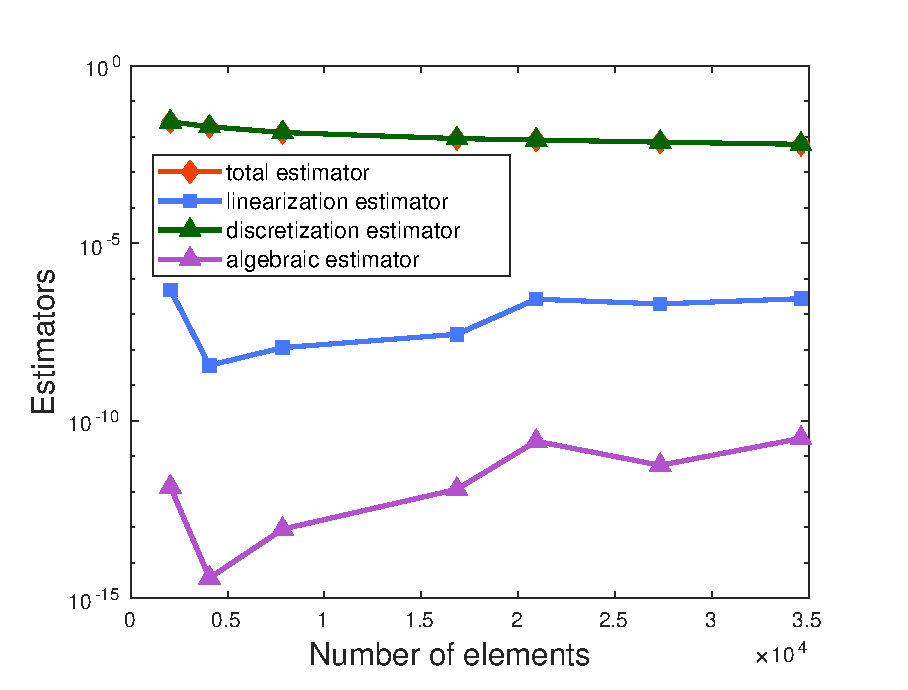
\includegraphics[width=\textwidth]{fig_article_chap_1/exact_resolution_convergence_estimator_number_elements.eps}    \end{minipage}\hfill
\begin{minipage}[c]{.333\linewidth}
   \centering
   \quad \small{Inexact Newton} \hspace{3 cm} \scriptsize{(\textcolor{midnightblue}{$\left\|\bR_{\mathrm{rel,alg}}^{\kk,\ii}\right\| \leq \left\|\bR_{\mathrm{rel,lin}}^{\kk,\ii}\right\|$, $\left\|\bR_{\mathrm{rel,lin}}^{\kk,\ii}\right\| \leq 10^{-10}$})}
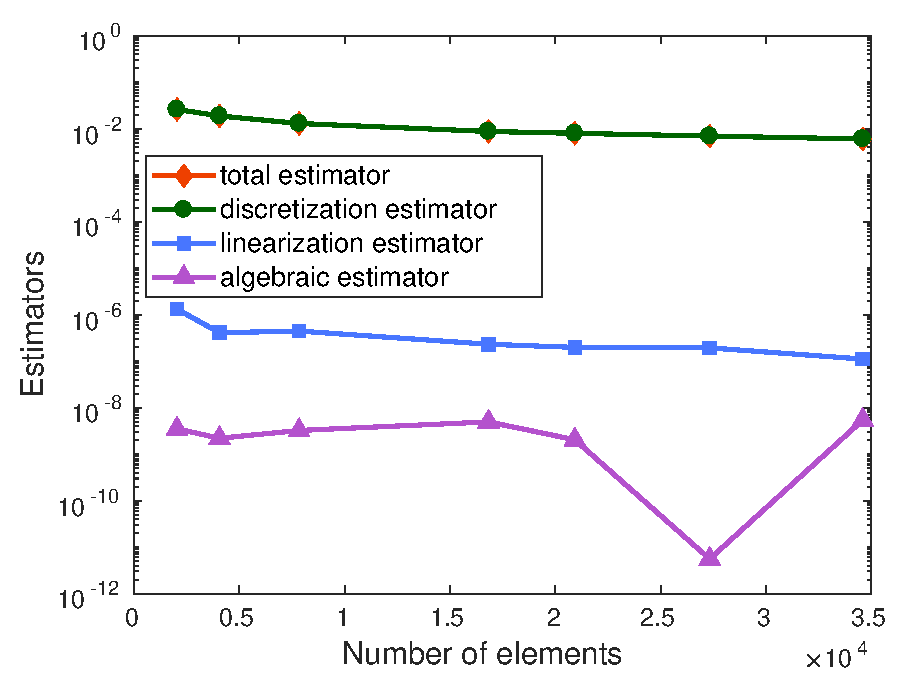
\includegraphics[width=\textwidth]{fig_article_chap_1/inexact_resolution_convergence_estimator_number_elements.eps}    

\end{minipage}\hfill
\begin{minipage}[c]{.33\linewidth}
   \centering
   \small{\small{Adaptive Inexact Newton} \hspace{3 cm} \scriptsize{\textcolor{midnightblue}{($\gammalin=10^{-1}$, $\gammaalg=10^{-1}$)}}}
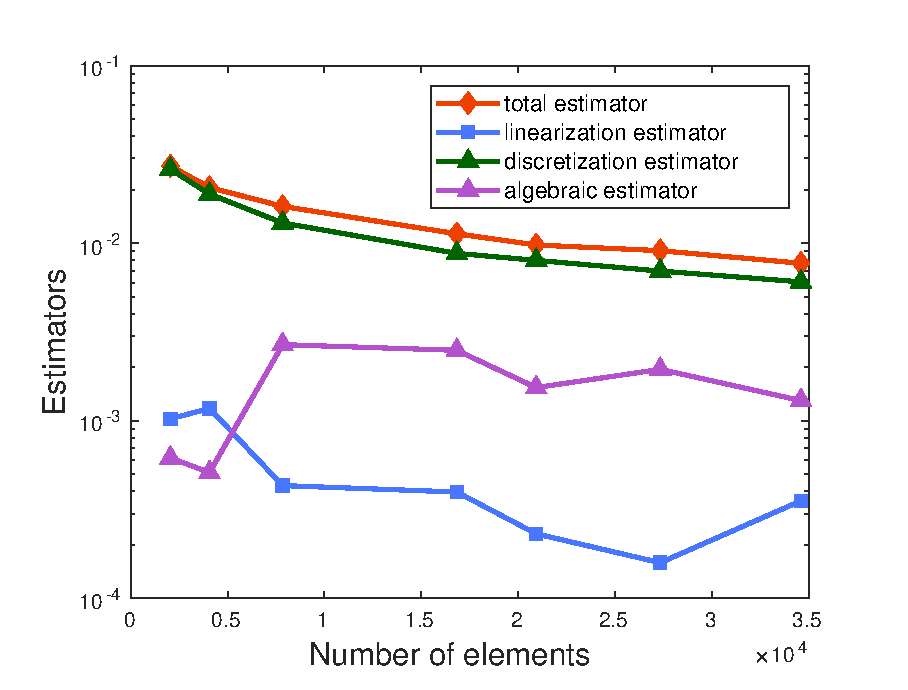
\includegraphics[width=\textwidth]{fig_article_chap_1/adapt_inexact_resolution_convergence_estimator_number_elements.eps}     
\end{minipage}
%\caption{Exact Newton(left), Inexact Newton(middle), adaptive inexact Newton(right)}
\end{figure}

\textcolor{red}{\textbf{Precision is preserved for adaptive inexact semismooth Newton method.}}


\end{frame}

\begin{frame}
\frametitle{Adaptivity}
\hspace{5.5 cm} Exact Newton/Adaptive inexact Newton \hspace{3.5 cm } 
%Inexact Newton
\begin{figure}
   \centering
%% 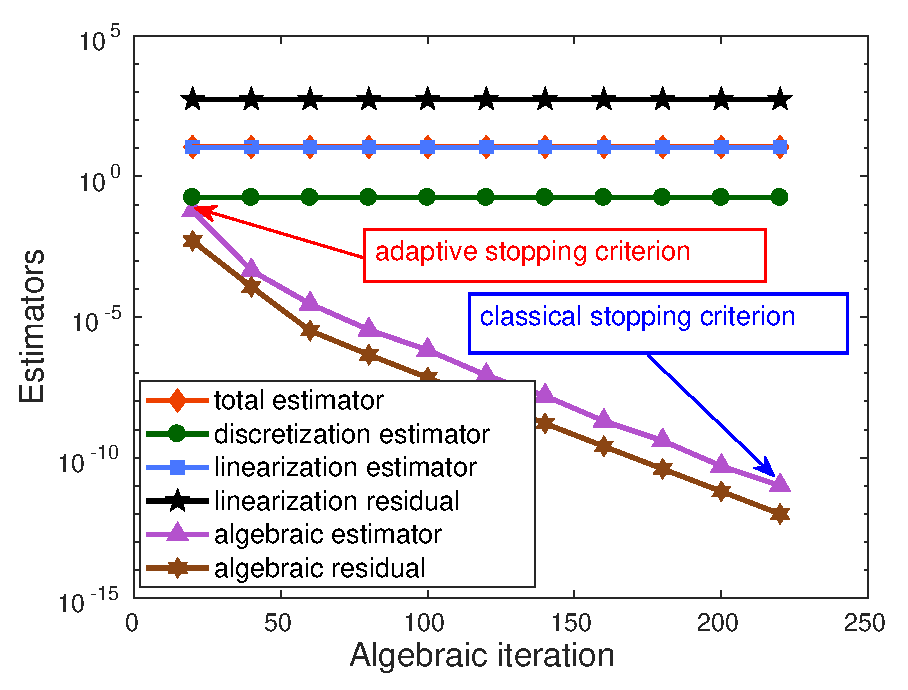
\includegraphics[width=0.50\textwidth]{fig_article_chap_1/exact_adapt_res_estimators_gmres_iter_first_newton_iter_Hmax_015.eps}    
\includegraphics[width=0.50\textwidth]{p2/Exact_P2_estimator_GMRES_per_1stNewton}
%% 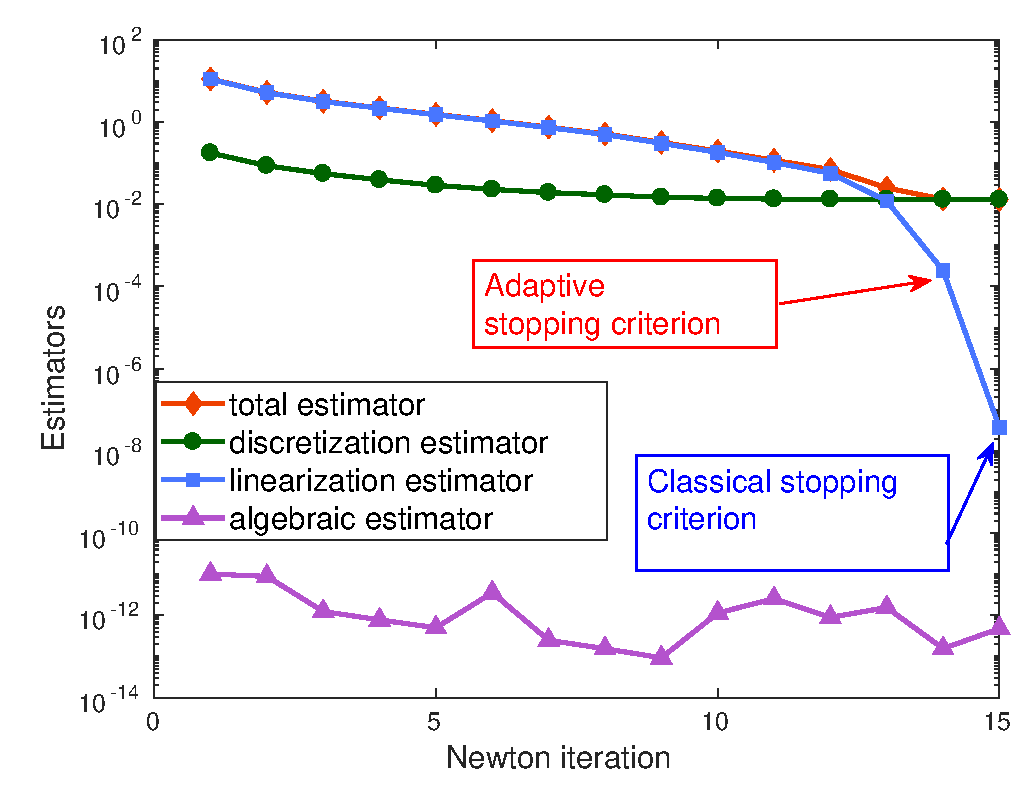
\includegraphics[width=0.49\textwidth]{fig_article_chap_1/exact_adapt_resolution_estimators_newton_iter_Hmax_015.eps}
\includegraphics[width=0.49\textwidth]{p2/Exact_P2_estimator_Newton_iter}
\end{figure}
\end{frame}

\begin{frame}
\frametitle{Overall performance}
\begin{figure}
\includegraphics[width=0.5\textwidth]{p2/P2_number_Newton_iter_per_elements}  
%% 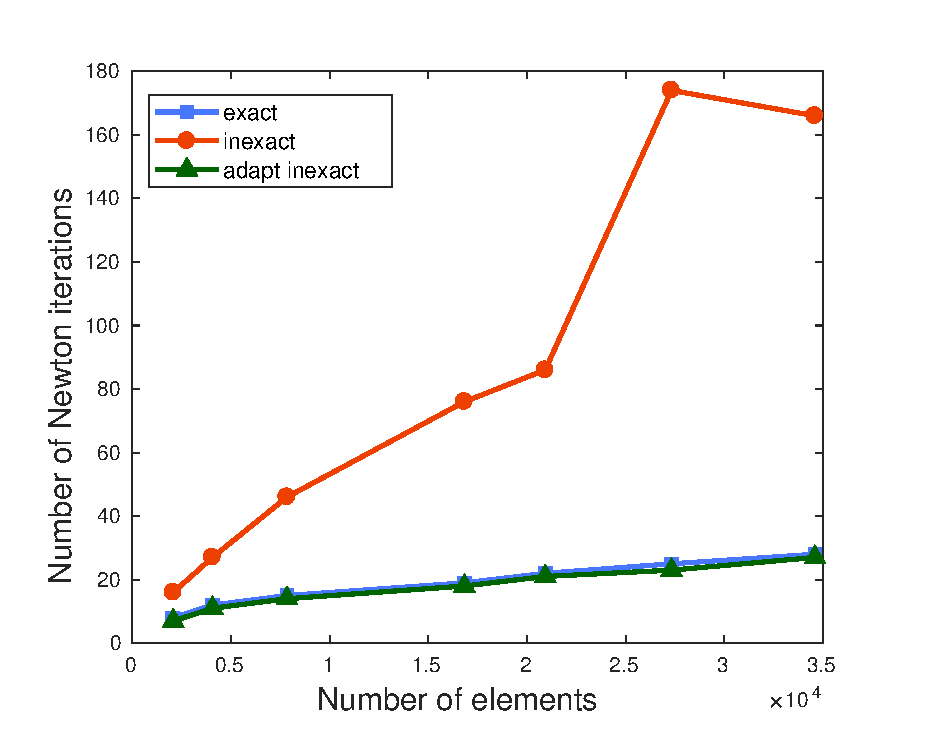
\includegraphics[width=0.46\textwidth]{fig_article_chap_1/comparison_three_methods_number_Newton_iter_number_elements.eps}
\quad  
%% 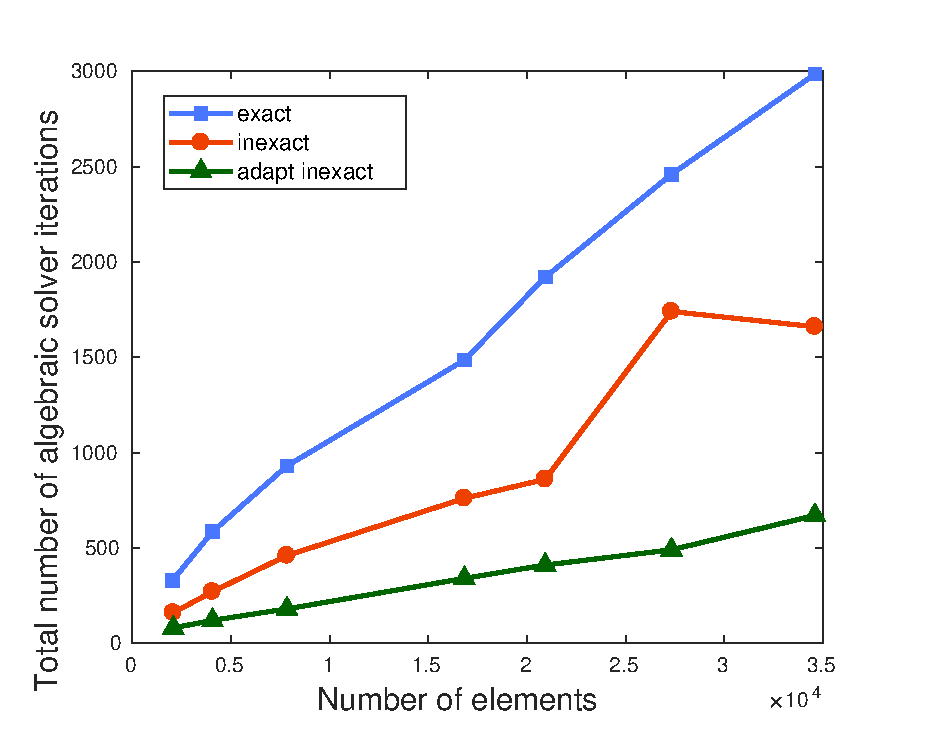
\includegraphics[width=0.49\textwidth]{fig_article_chap_1/comparison_three_methods_total_number_Newton_Gmres_iter_number_elements.eps}
 \includegraphics[width=0.46\textwidth]{P2_tot_number_GMRES_iter_per_elements}
\end{figure}
\begin{thebibliography}{10}
 \scriptsize{
 \bibitem{Dabaghi:Martin:Vohralik:2020}
 {\sc J.~Dabaghi, V.~Martin, M.~Vohral\'{i}k}, Adaptive Inexact Semismooth Newton Methods for the
Contact Problem Between Two Membranes.
\em{Journal of Scientific Computing} (2020).
}
 \end{thebibliography}
\end{frame}
%%%%
%% \begin{frame}
%%   \vspace*{0.1 cm}
%%   \hspace{0.5 cm}\textcolor{red}{\textbf{Effectivity indices:}} $\mathrm{I}_{\mathrm{eff}} \egaldef \frac{\eta^{\kk,\ii}}{\tnorm{\bu-\bu_h^{\kk,\ii}}_{\Omega}}$ \hspace{3 cm} \textcolor{red}{\textbf{contact estimator}}
%% \vspace*{-0.2 cm}
%%   \begin{figure}
%% \includegraphics[width=0.46 \textwidth]{p2/P2_effectivity_index_three_methods}    
%% %% 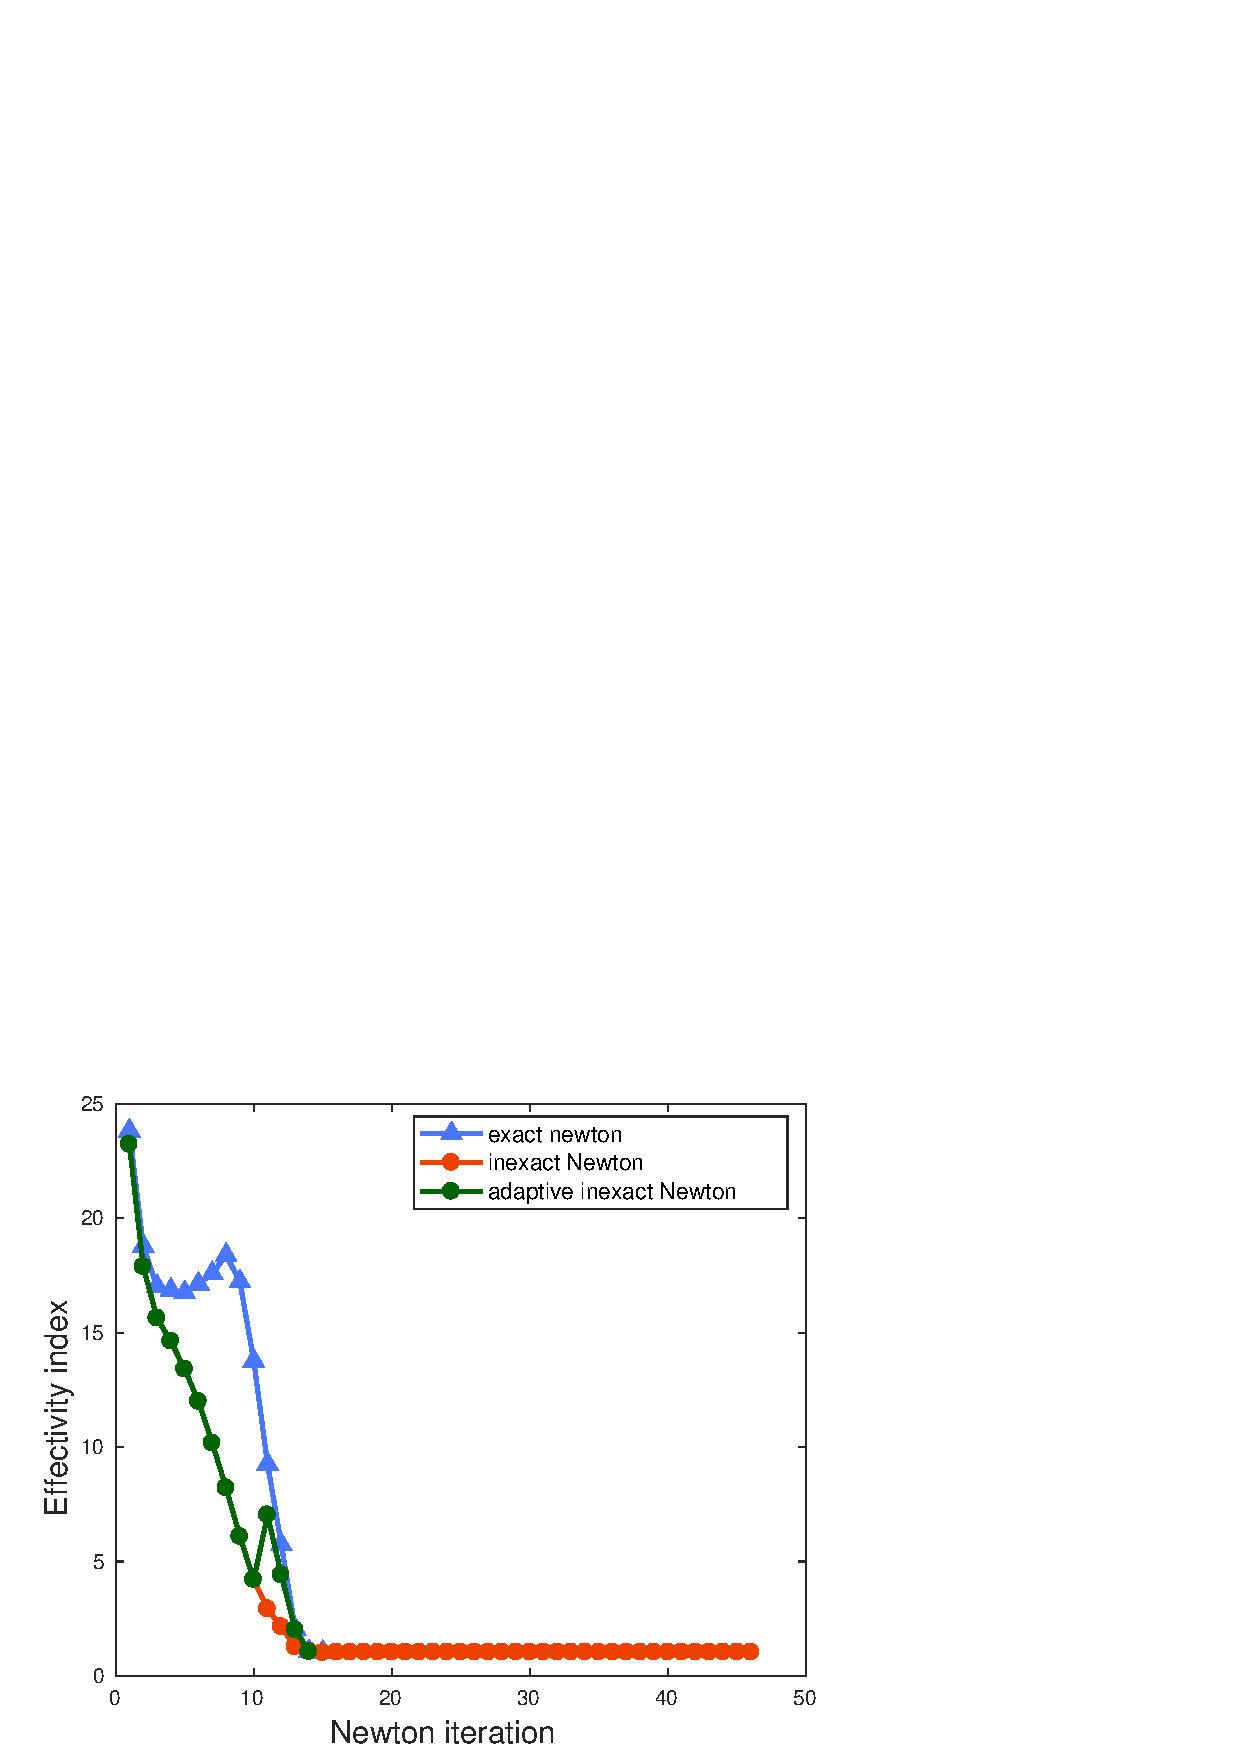
\includegraphics[width=0.46 \textwidth]{fig_article_chap_1/effectivity_index_3_methods_Hmax_015.pdf}
%% \quad 
%% \includegraphics[width=0.49 \textwidth]{fig_article_chap_1/modif_fig_contact_estimator_hmax0,09_Dt0,001_tt180}
%% \end{figure}
%% \begin{thebibliography}{10}
%%  \scriptsize{
%%  \bibitem{Dabaghi:Martin:Vohralik:2020}
%%  {\sc J.~Dabaghi, V.~Martin, M.~Vohral\'{i}k}, Adaptive Inexact Semismooth Newton Methods for the
%% Contact Problem Between Two Membranes.
%% \em{Journal of Scientific Computing} (2020).
%% }
%%  \end{thebibliography}
%% \end{frame}


%%%%%%%%%%% CHAP 3

\section{Extension to unsteady problems}
\subsection{}

\input{Part3}
%

%% CONCLUSION
\section{Conclusion}
\subsection{}

\input{Conclusion.tex}



% \bibliographystyle{plain}
% \bibliography{diphasique_biblio}
\end{document}



